% Section 4 -- Task 2: PPO. Figures: results/task2_ppo/analysis/figures/ (analysis/task2_report_stats.py).
\section{Task 2: Proximal Policy Optimization}
\label{sec:ppo}
We continue PPO from the supplied midpoint (Qwen2.5-1.5B LoRA policy, 0.5B LoRA critic, frozen reward model $r_\psi$) for 20 updates (one prompt, two epochs, LR $3{\times}10^{-6}$, GAE $\gamma{=}1,\lambda{=}0.95$, $\epsilon{=}0.2$, $\beta_{\text{KL}}{=}0.1$). Ablations fork 8-update runs from the identical state with common random numbers over $\epsilon\in\{0.05,0.2,0.5\}$ and $\beta_{\text{KL}}\in\{0,0.1,0.2\}$. All conditions use the same 200 held-out prompts with paired-bootstrap 95\% CIs (Table~\ref{tab:ppo}).

\begin{table}[h]
\centering\small
\caption{Training statistics (mean $\pm$ std over updates) and held-out reward change vs.\ the midpoint ($r_\psi{=}1.533$; 95\% paired-bootstrap CI). $^\dagger$The three $\epsilon$ forks are bit-identical and share a row (equal to $\beta{=}0.1$).}
\label{tab:ppo}
\setlength{\tabcolsep}{2.4pt}
\begin{tabular}{@{}lcccccccc@{}}
\toprule
Run & $\mathcal{L}_V$ & Clip frac. & $\max|\rho{-}1|$ & $\hat D_{\text{KL}}$ ($10^{-4}$) & $r_\psi$ (train) & Entropy & Length & Held-out $\Delta r_\psi$ \\
\midrule
Standard (20 upd.) & $4.30\pm1.45$ & 0 & 0.078 & $-0.1\pm5.1$ & $1.19\pm1.37$ & $1.04\pm0.51$ & $241\pm186$ & $+.034$ [$-.034,.106$] \\
$\epsilon\in\{.05,.2,.5\}^\dagger$ & $5.47\pm1.11$ & 0 & 0.031 & $-0.3\pm6.7$ & $0.86\pm1.05$ & $0.87\pm0.43$ & $224\pm239$ & $+.002$ [$-.055,.068$] \\
$\beta_{\text{KL}}=0$ & $5.59\pm1.14$ & 0 & 0.027 & $-1.2\pm8.8$ & $0.73\pm1.18$ & $0.86\pm0.43$ & $219\pm243$ & $+.019$ [$-.072,.110$] \\
$\beta_{\text{KL}}=0.2$ & $5.79\pm1.11$ & 0 & 0.029 & $+2.6\pm5.5$ & $0.82\pm1.14$ & $0.84\pm0.42$ & $219\pm243$ & $+.051$ [$-.040,.144$] \\
\bottomrule
\end{tabular}
\end{table}

\subsection{Baseline and Critic Dynamics}
The surrogate loss is negligible ($|\mathcal{L}_\pi|\sim10^{-4}$) because $\rho\approx1$, so learning hinges on the critic, which fails. Explained variance is negative in 20/20 updates (median $-5.3$), and the mean value loss (4.30) exceeds the reward variance (2.16), so $V_\phi$ is worse than a constant predictor. With terminal rewards and $\gamma{=}1$, GAE accumulates $\delta_t=V_{t+1}-V_t$ inside each response, so an uncalibrated critic adds token-wise noise to every advantage, which whitening cannot remove. This shows up as an erratic policy-gradient norm (CV 0.78) and a critic gradient that exceeds its clip by 36--287$\times$ in every update (Fig.~\ref{fig:app_std}). One trajectory per update is too little data to fit a length-dependent value function.

\subsection{RQ1: Clipping ($\epsilon$)}
The clip binds only when $|\rho-1|>\epsilon$, but $\max|\rho-1|=0.031$ across all $\epsilon$ forks. The clip fraction is therefore 0 in every update, the clipped and unclipped gradients coincide, and the three forks are bit-identical in training and held-out metrics (Fig.~\ref{fig:ppo_clip}). A cached-batch probe that seemed to show clipping (0.55/0.34/0.18) had used mismatched prompts. Corrected, it gives 0.108/0.0085/0.0056, equal to a noise-only floor (0.112/0.0084/0.0057) from bf16-versus-fp16 numerics. The reason is the step size: with one prompt and two epochs, $\rho\neq1$ arises only after a single Adam step at LR $3{\times}10^{-6}$, which moves probabilities by at most 3\%. PPO here is a policy gradient inside the trust region, and $\epsilon$ cannot affect stability, entropy or reward.


\begin{figure}[!htbp]\centering
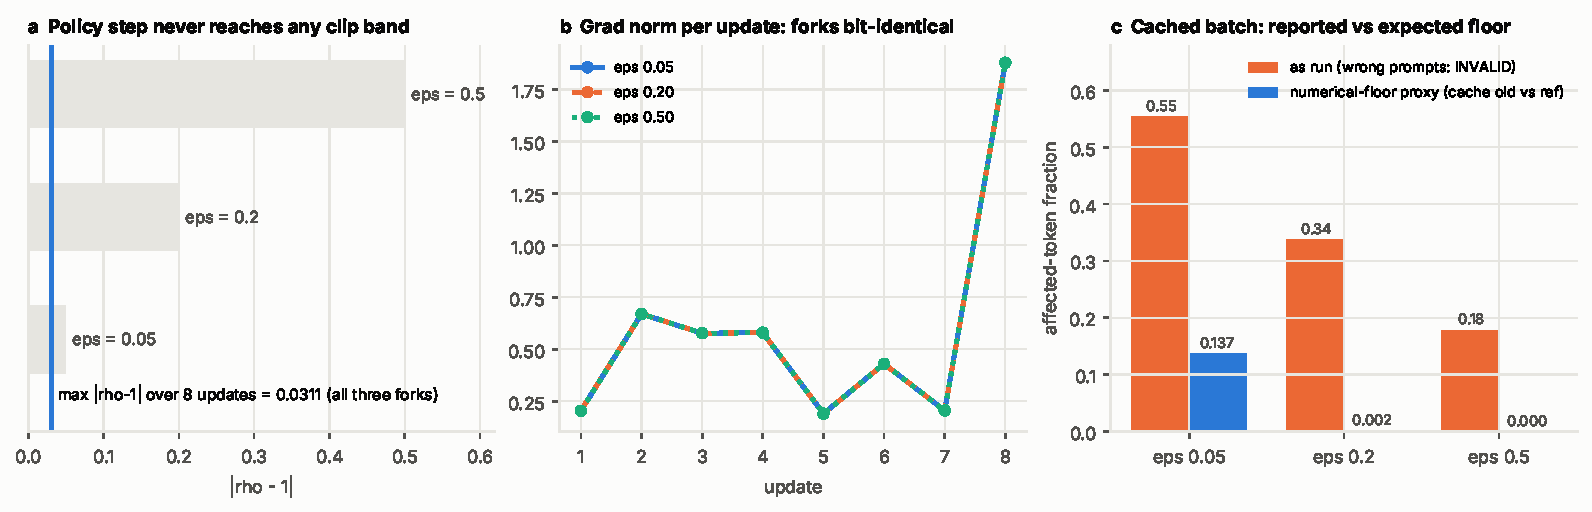
\includegraphics[width=\linewidth]{fig2_clipping_study.pdf}
\caption{Clipping. (a) $\max|\rho-1|$ (0.031) never reaches any band. (b) Gradient norms of the three $\epsilon$ forks coincide. (c) Cached-batch affected fraction before and after the prompt correction; the corrected value equals the numerical floor.}
\label{fig:ppo_clip}
\end{figure}

\subsection{RQ2: KL Pressure ($\beta_{\text{KL}}$)}
Because update 1 is identical across forks, later differences are caused by $\beta$. KL and entropy diverge first (update 2, on identical sampled tokens), then reward and length (update 3). Fluency is unchanged (distinct-2 0.931--0.935 vs.\ 0.934). This order reflects measurement sensitivity rather than a cascade: log-probability statistics register $10^{-4}$ changes, while reward moves only when a sampling decision flips, an $O(1)$ bifurcation whose winner is arbitrary. The ordering is therefore not monotone in $\beta$ (Fig.~\ref{fig:ppo_kl}). The penalty never binds: $\beta|\mathrm{KL}_{\text{seq}}|\le0.02$ ($<$2\% of the reward s.d.), and $\nabla\mathrm{KL}$ vanishes at the reference. Even $\beta{=}0$ shows no drift or entropy collapse, so these runs cannot show that the penalty \emph{prevents} collapse, only that it was inactive.


\begin{figure}[!htbp]\centering
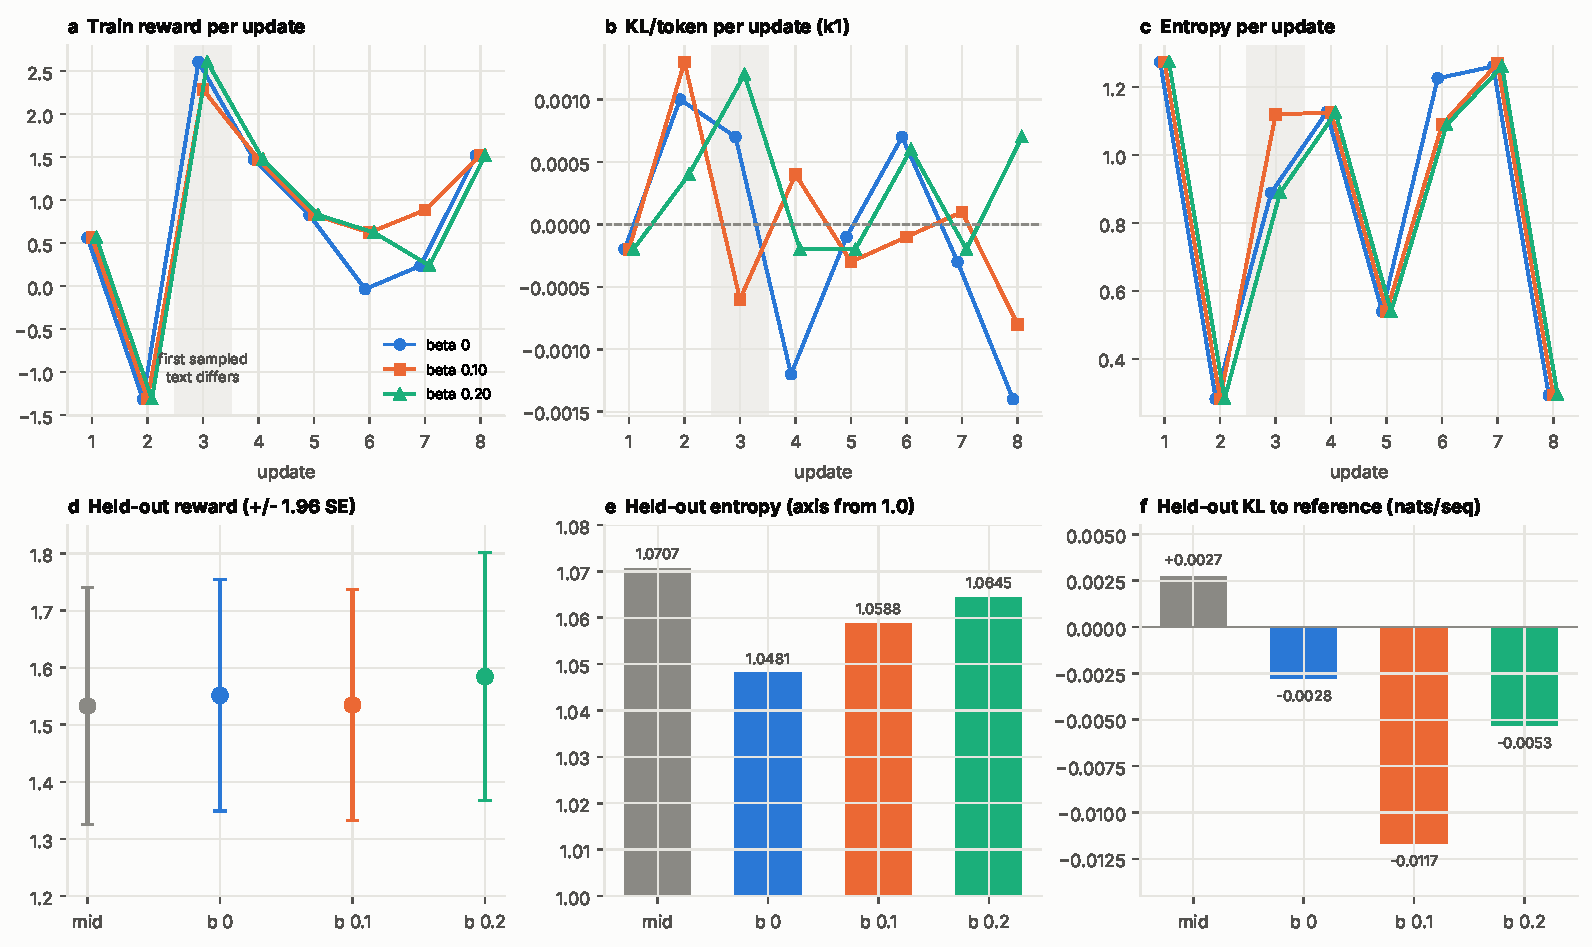
\includegraphics[width=\linewidth]{fig3_kl_study.pdf}
\caption{KL forks. (a--c) Training reward, KL and entropy; the grey band marks the first update whose sampled text differs. (d--f) Held-out reward ($\pm1.96$ SE), entropy and KL; no condition separates from the midpoint.}
\label{fig:ppo_kl}
\end{figure}

\subsection{RQ3: Reward Reliability and Over-optimization}
No over-optimization is detectable because the policy never drifts. All held-out CIs include zero, $|\mathrm{KL}_{\text{seq}}|\le0.012$ nats, and 63--67\% of responses match the midpoint verbatim. The proxy is nonetheless fragile. It has 0.674 pairwise accuracy, a length correlation of 0.34, and a per-sample noise floor (0.126) larger than any mean effect. Right-truncating prompts at 256 tokens (17.5\% of the evaluation set) removes the assistant header and lowers reward by 2.14 ($p{<}10^{-4}$; Fig.~\ref{fig:app_rel}). Two same-seed pairs illustrate this. On idx 178, reward rises from $-0.13$ to $+1.11$ for a genuinely more helpful, though three times longer, answer. On a truncated translation prompt (idx 72), it rises from $+0.15$ to $+2.23$ for a looping, unterminated output (distinct-2 $0.69\to0.57$). Both are sampling bifurcations, not learned exploits, but they expose the biases (length, tolerated repetition, truncation) that stronger optimization would exploit first.

\paragraph{Limitations.} The study uses a single seed and one prompt per update. The standard-run adapter used for the held-out evaluation was regenerated by retraining, so its identity with the original is assumed.
